% This chapter includes
% 3. Analysis procedures
%    3.1 Data sets and MC samples
%        3.1.X sub-sections for samples
%    3.2 Trigger
%    3.3 Physics objects reconstruction and identification
%        3.3.X sub-sections for physics objects

\chapter{Analysis Procedures}

In this chapter, the analysis procedures of the search for $Z'$ decaying into $Z$h in $llbb$ final state are reported. The data sets and Monte Carlo (MC) samples we used in this analysis will be indicated. Physics objects reconstruction and event selections are also introduced. Moreover, background yields and the effects of systematic uncertainties will be demonstrated in the end of this chapter.

\section{Monte Carlo Samples and Data sets}

\subsection{Signal MC}
As introduced in section 1.2.3, the signal hypothesis is HVT model B benchmark. The heavy resonance ($Z'$) is tested using a wide set of masses from 800 GeV to 2000 GeV, one masspoint every 100 GeV (Table~\ref{tab:TableSignalMC}). The signal is simulated by MadGraph5\_aMC$@$NLO\cite{MG5} in LO mode, as a narrow spin-1 neutral resonance and is forced to decay in the $Z'\rightarrow Zh\rightarrow llqq$ channel. Showering and hadronization are performed with PYTHIA6\cite{PYTHIA}.
\begin{figure}[hbtp]
  \begin{center}
    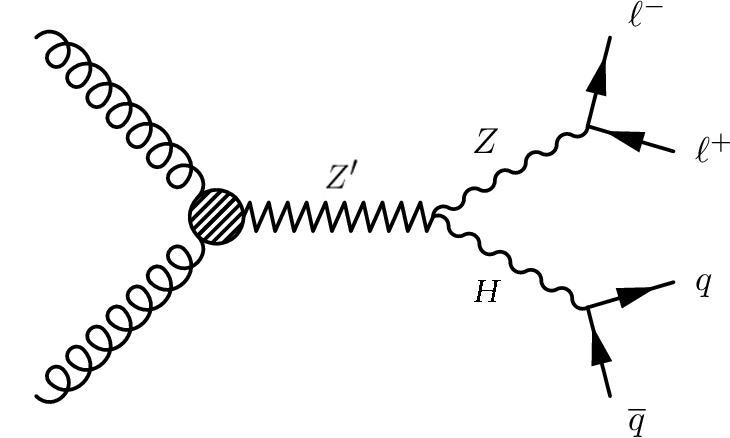
\includegraphics[width=0.4\textwidth]{figure/CH3/ZPrimeTo2l2q.png}
  \end{center}
  \caption{\label{fig:ZPrime2l2q}Feynman diagram for $Z'\rightarrow Zh \rightarrow 2l2q.$}
\end{figure}
\begin{center}
  \begin{table}
    \begin{center}
      \begin{tabular}{|c|c|c|}
        \hline
        Sample & Number of Processed Events & $\sigma_{LO}$(pb) \\ \hline
        ZPrime\_ZH\_lljj\_M800-MADGRAPH & 10710 & 0.00685367 \\ \hline
        ZPrime\_ZH\_lljj\_M900-MADGRAPH & 10209 & 0.00485861 \\ \hline
        ZPrime\_ZH\_lljj\_M1000-MADGRAPH & 19997 & 0.003263 \\ \hline
        ZPrime\_ZH\_lljj\_M1100-MADGRAPH & 9370 & 0.00217483 \\ \hline
        ZPrime\_ZH\_lljj\_M1200-MADGRAPH & 10710 & 0.00145484 \\ \hline
        ZPrime\_ZH\_lljj\_M1300-MADGRAPH & 9369 & 0.000979745 \\ \hline
        ZPrime\_ZH\_lljj\_M1400-MADGRAPH & 10497 & 0.000664783 \\ \hline
        ZPrime\_ZH\_lljj\_M1500-MADGRAPH & 19999 & 0.000454339 \\ \hline
        ZPrime\_ZH\_lljj\_M1600-MADGRAPH & 8950 & 0.000312541 \\ \hline
        ZPrime\_ZH\_lljj\_M1700-MADGRAPH & 9369 & 0.000216282 \\ \hline
        ZPrime\_ZH\_lljj\_M1800-MADGRAPH & 10708 & 0.000150398 \\ \hline
        ZPrime\_ZH\_lljj\_M1900-MADGRAPH & 10498 & 0.000105039 \\ \hline
        ZPrime\_ZH\_lljj\_M2000-MADGRAPH & 19999 & 7.36377e-05 \\
        \hline
      \end{tabular}
    \end{center}
    \caption{\label{tab:TableSignalMC}Signal samples used in the analysis.}    
  \end{table}
\end{center}
\newpage
\subsection{Background MC}
Since we are looking for new resonances decaying in semi-leptonic final state, the background samples of this analysis are originated by all SM events with two leptons and at least one jet as final state. The dominant background contribution is the produciton of Z boson with jets. This Z+jets sample is produced by MADGRAPH. In the matrix element level, the Z boson is forced decaying into two leptons, and further this sample is divided into two samples depending on the Z $p_{T}$, higher than 100 GeV or between 70 and 100 GeV. The contribution of events with Z $p_{T}$ less than 70 GeV is negligible due to further cut on the objects $p_{T}$ in the selection criteria.

The second dominant source of background is $t\bar{t}$ production. Both of the two top quarks decay into all leptonic final state (top decays into a W boson and a b quark first) which gives two leptons, neutrinos and two b-jets. This sample is generated by POWHEG\cite{POWHEG}.

Other sources of background considered are SM di-boson productions (WW, WZ and ZZ) generated by PYTHIA6. All the background samples are required to pass phase-space cuts, $p_{T}^{ll} > $60 GeV and 60$ < M_{ll} < $120 GeV. Related statistics are reported in Table~\ref{tab:TabBkgMC}.

\begin{center}
  \begin{table}[h]
    \begin{center}
      \begin{tabular}{|c|c|c|}
        \hline
        Sample & Number of Processed Events & $\sigma_{NLO}$(pb) \\ \hline
        DYJetsToLL\_PtZ-70To100 & 11764538 & 63.5 \\ \hline
        DYJetsToLL\_PtZ-100 & 12511326 & 39.4 \\ \hline
        TTTo2L2Nu2B & 10783509 & 25.8 \\ \hline
        WW & 7759752 & 56.0 $\pm$ 2.3 ($\pm$ 0.3) \\ \hline
        WZ & 9910267 & 22.4 \\ \hline
        ZZ & 9769891 & 7.6 $\pm$ 0.3 ($\pm$ 0.3)\\
        \hline
      \end{tabular}
    \end{center}
    \caption{\label{tab:TabBkgMC}Background samples used in the analysis.}    
  \end{table}
\end{center}

\subsection{Data Samples}
In this analysis, the full CMS data collected in 2012 is used, corresponding to the integrated luminosity of 19.7 fb$^{-1}$ at center-of-mass energy $\sqrt{s} = $8 TeV. For each lepton channel, there are four datasets. All datasets are collected with a double muon or a double electron trigger, as explained in detail in the next section. The trigger algorithm employed for the electron samples doesn't use any information from the tracker but only the energy deposite in the ECAL. This expedient is implemented in order to avoid any possible inefficiencies due to the presence of two tracks very close to each other when the Z is highly boosted and its decay products are very collimated. Such a trigger is contained in the Photon/DoublePhotonHighPt dataset. The full dataset names are listed in Table~\ref{tab:TabDataSet}.

\begin{center}
  \begin{table}[h]
    \begin{center}
      \begin{tabular}{|c|c|}
        \hline
        AOD Sample & Luminosity (pb$^{-1}$) \\ \hline
        DoubleMu/Run2012A-22Jan2013-v1 & 876.225 \\ \hline
        DoubleMuParked/Run2012B-22Jan2013-v1 & 4409 \\ \hline
        DoubleMuParked/Run2012C-22Jan2013-v1 & 7017 \\ \hline
        DoubleMuParked/Run2012D-22Jan2013-v1 & 7369 \\ \hline
        Photon/Run2012A-22Jan2013-v1 &  876.225 \\ \hline
        DoublePhotonHighPt/Run2012B-22Jan2013-v1 & 4412 \\ \hline
        DoublePhotonHighPt/Run2012C-22Jan2013-v1 & 7055 \\ \hline
        DoublePhotonHighPt/Run2012D-22Jan2013-v1 & 7369 \\
        \hline
      \end{tabular}
    \end{center}
    \caption{\label{tab:TabDataSet}Data sets used in this analysis.}    
  \end{table}
\end{center}

\section{Trigger}




